% Chapter Implementation
%

\chapter{Implementation}

The program and modules developed in this thesis enable the building and simulation
of a full mouse brain model relaying on point neuron models. Such a model must be built by
reconstructing parts from experimental data.
Allen Institute for Brain Science and the Blue Brain Project provide such data.
To this aim, the pipeline of large scale data-driven simulations with neuronal simulation tool NEST is investigated.
In order to carry on the simulation, an efficient data format is defined, the circuit generation scripts are adapted to
run on a larger scale, the generated circuit is validated and NEST is extended to load the new data format.

\section{Data formats}
\label{sec:dataformats}
A point neuron model contains point neurons and connections (synapses) between the point neurons.
The same point neuron model (conductance based exponential integrate-and-fire neuron model \cite{brette2005adaptive}) and synapse model (Tsodyks synapse model containing synaptic short-term depression and short-term facilitation \cite{tsodyks1997neural, fuhrmann2002coding}) are used for all neurons and synapses, respectively.
The neurons and synapses are characterized by parameters.
Each neuron is defined by a given set of parameters.
Besides the parameters, the synapses contain pre-synaptic and post-synaptic neuron ids.
To store the circuit in files, two different data formats are defined.
The first data format defines the storage of all neuron parameters.
The second data format defines the storage of synapse parameters and pre-synaptic and post-synaptic neuron ids.

The data format (see Figure \ref{fig:file:neuron}) for the neurons and the synapses follow two different concepts.
The neuron data format contains multiple datasets containing the neuron parameters.
By definition, all datasets have, the same length. This length defines the number of neurons.
The neuron parameters of neuron $i$ are stored in the i-th row of each parameter dataset.
\begin{figure}[ht!]
   	\begin{center}
        \subfigure[The neuron file contains a dataset for each parameter.
        Each dataset is a one dimensional array of \emph{H5T\_NATIVE\_FLOAT} values.]{%
            \label{fig:file:neuron}
            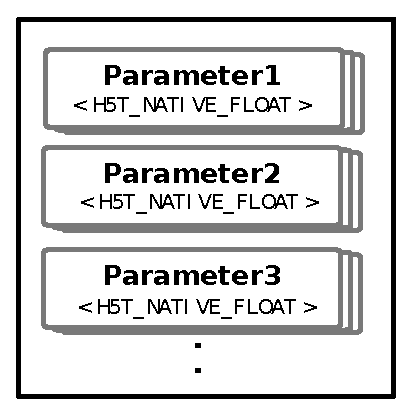
\includegraphics[scale=0.6]{pictures/hdf5_neuron_format.eps}
        }
        \hspace{0.5cm}
        \subfigure[The synapse file contains two datasets: \emph{neuron} and \emph{syn}.
		\emph{neuron} groups the pre-synaptic neuron ids with references to the \emph{syn} dataset.
		\emph{syn} contains post-synaptic neuron ids and synapse model parameters.]{%
            \label{fig:file:synapse}
            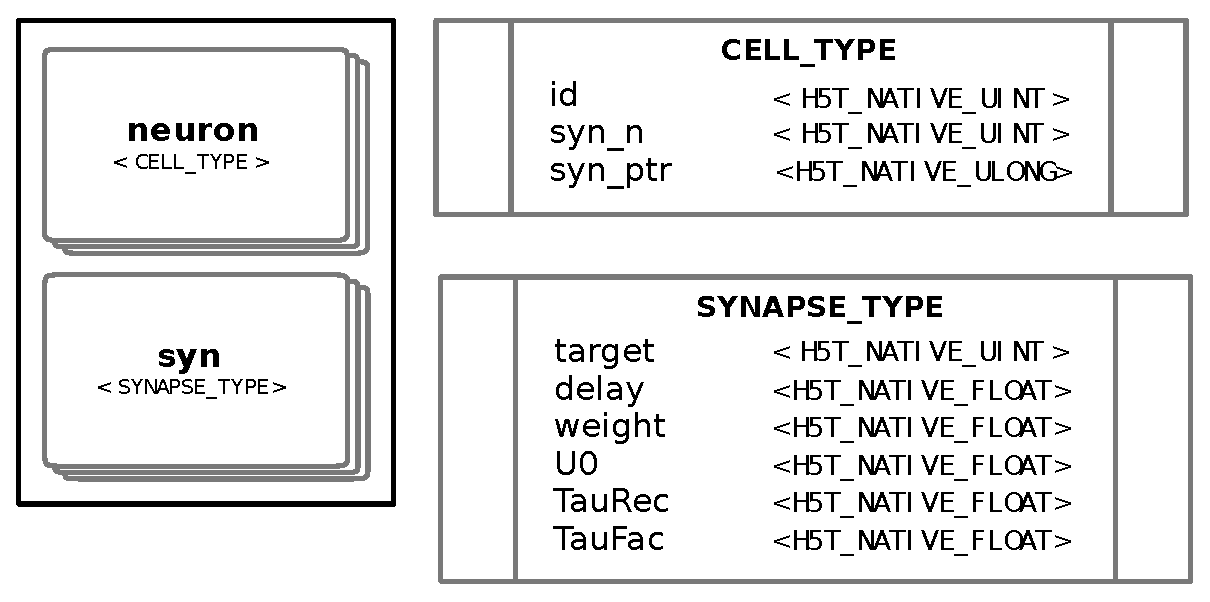
\includegraphics[scale=0.41]{pictures/hdf5_syn_format.eps}
       }
    	   \end{center}
    	\caption[Data formats of neurons and synapses with their related datasets and data types]{%
        The diagrams show the data formats of neurons and synapses with their related datasets and data types.
     }%
   \label{fig:file}
   \end{figure}
   
The synapse data format (see Figure \ref{fig:file:synapse}) contains two datasets. For each synapse, the datasets generally contain
a pre-synaptic neuron id, a post-synaptic neuron id and a set of parameters.
To reduce the amount of data the pre-synaptic neuron ids are grouped together in one \emph{neuron} dataset.
This is feasible, because
the number of synapses is greater than the number of pre-synaptic neurons (around $10,000$ synapses per pre-synaptic neuron).
The dataset contains an array of pre-synaptic neuron ids (\emph{id}) with references (\emph{syn\_n} and \emph{syn\_ptr}).
The \emph{syn\_ptr} value defines the related starting index in the \emph{syn} dataset,
and \emph{syn\_n} defines the number of related following entries.
The \emph{syn} dataset contains the post-synaptic neuron ids and a set of parameters.
Both datasets use a compound data type to store different data types in a single dataset.


\section{Circuit generation}
The mouse brain model is generated from experimental data of the Allen Brain Atlas and
the Blue Brain Project recipe.
At first a point neuron cloud is generated with all its parameters.
After that the synapses are generated.
The described circuit generation (see Chapter \ref{sec:allen}) calculates the synapses for a given point neuron cloud.
The point neuron cloud generation is already given and can be used for the full circuit.
The already existing python scripts can generate the connections for up to $0.3$ percent of the full mouse brain model.
These scripts are developed to fit on local laptops.
A full mouse brain model generation requires more resources and computation power, in order to move forward, larger machines have to be used.
The circuit generation should be ported on the Blue Brain 4 super computer.
In order to use the resources provided by the super computer, a new implementations needs to be developed. 
Rewriting the sequential python scripts to a hybrid C++ application requires a parallel implementation of the algorithms.


%%insert somewhere
%Unfortunately all injections from these experiments do not
%cover the whole brain. So there are neurons which are not injected
%by any experiment. Therefore all neurons which are not injected should use the projection
%from the nearest injection.


\subsection{Long range connections}
The mouse brain model contains long range connections.
These long range connections are synapses between neurons in different brain regions.
Cross regions connections probabilities from the Allen Brain Atlas are evaluated and 
mapped on the point neuron cloud. Synapses are generated based on these probabilities.
Algorithm \ref{alg2} is mainly based on three nested \emph{for} loops.
% long range connections generation ,.. do you need all these words?
The outer loop iterates over the injection experiments, the inner one over voxels, which are injected by the experiment, and the third
one over neurons inside the voxel.
Besides a \emph{if} condition in the voxel iteration, there are no dependencies between the iterations.
The if condition compares the total injection densities.
It only regenerates the connections for the voxel if the current
experiment injects less than the previous experiments (less injection means more precise projections).
For a parallel implementation (see Figure \ref{fig:longrangParallel}) this dependency has to be avoided.
To overcome the dependency, the best experiment (the best experiment per voxel is the experiment with the smallest injection which still injects the current voxel) per voxel is chosen and calculated beforehand.
Thus, the loop over the voxels moves outside the loop over the experiments.

Once the used voxels are identified the number of generated synapses can be calculated, based on the
number of neurons inside the voxels and the hard-coded number of synapses per neuron, specified by model properties.
Thus, the HDF5 file and the \emph{syn} dataset is created before the voxel iterations.
The iterations of the loop over the voxels are distributed on the ranks.
Inside the iteration over all neurons, the sequential part of the algorithm can be applied.
\begin{figure}[ht!]
\centering
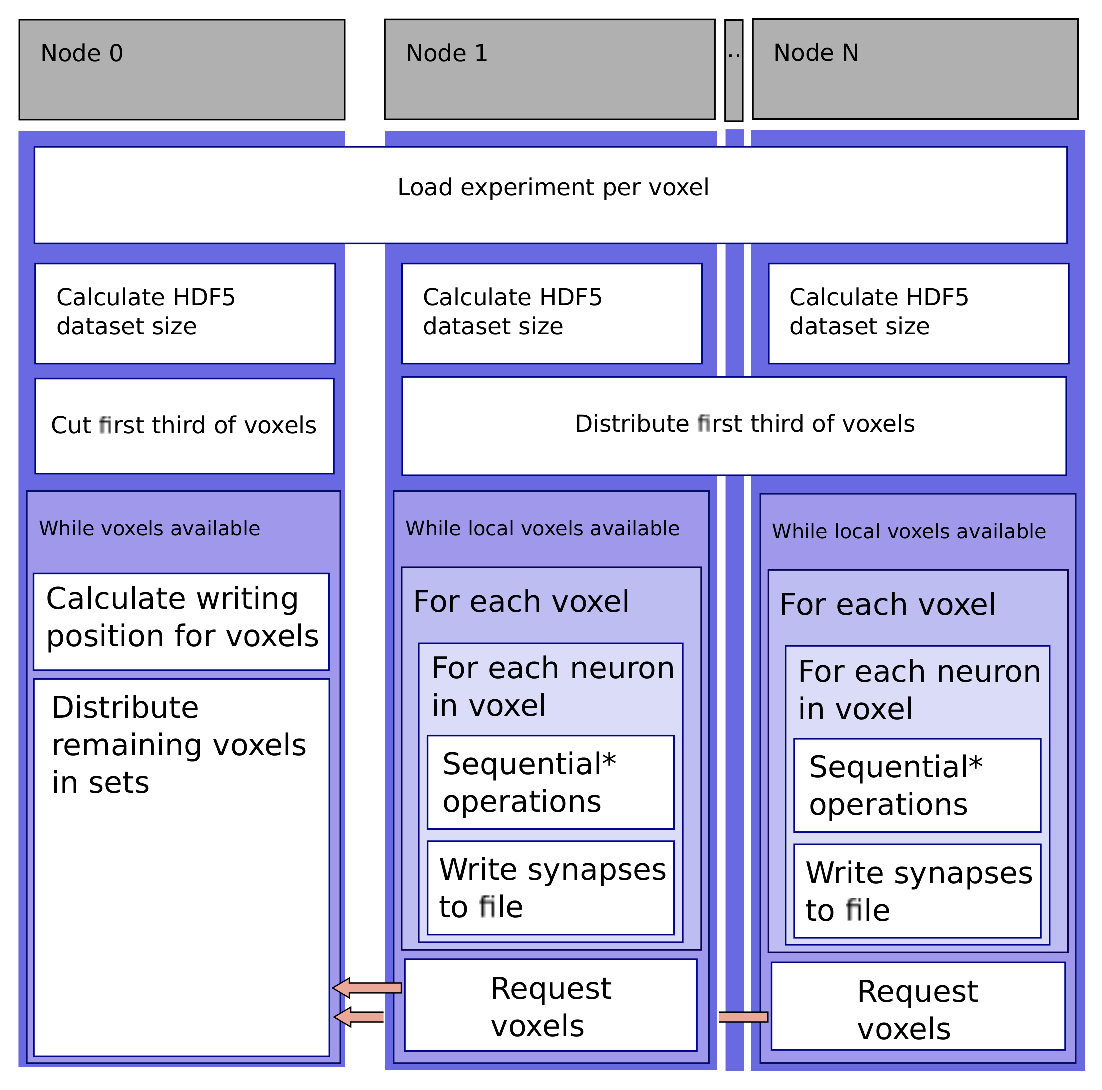
\includegraphics[scale=0.5]{pictures/longRange_parallelAlg.eps}
\caption[Task distribution between the ranks for the long range connections generation]{Task distribution between the ranks for the long range connections generation. It illustrates which tasks are distributed between which ranks.}
\label{fig:longrangParallel}
\end{figure}

\emph{Rank 0} is selected as the master rank. It does not participate in the iterations.
It manages the dynamic distribution of the voxels to the other ranks and 
assigns writing positions to the pre-synaptic neurons. Thus, each rank receives the 
voxel information and the writing positions,
where it has to write its data to the HDF5 datasets.
\begin{figure}[ht!]
\centering
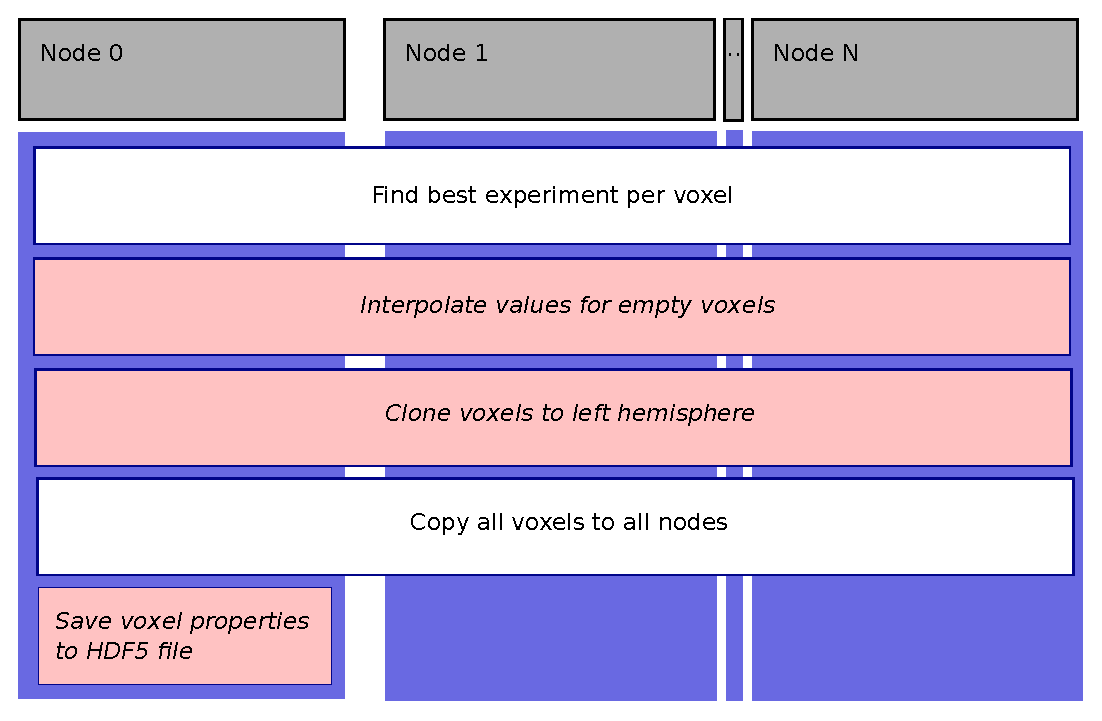
\includegraphics[scale=0.5]{pictures/longRange_BestExp_parallelAlg.eps}
\caption{Subtasks of the above listed \emph{Load experiment per voxel} task}
\label{fig:longrangeLEPV}
\end{figure}

Figure \ref{fig:longrangParallel} illustrates the workflow of all ranks.
Task \emph{Load experiment per voxel} from Figure \ref{fig:longrangParallel} contains several subtasks.
It generates the voxel datasets, which are later distributed.
Manipulations of the generation affect mostly this part.
Thus, the part enables modifications of the applied functionalities. 
Further, the whole function can be skipped by loading the voxel information from file (see Appendix \ref{file:voxelinfo}).
Figure \ref{fig:longrangeLEPV} shows the subtasks.
The red tasks are optional and can be enabled via command line arguments (see Table \ref{tab:longrangeargs}).
In the first task \emph{Find best experiment per voxel} each rank loads a set of experiments.
Iteratively the experiment with the smallest total injection density is assigned to each voxel.
Afterwards a MPI reduction function returns the smallest value for each voxel on
each rank.
However, there are regions which were not injected by any experiment available.
Thus, there is no connection information available for the internal neurons.
To overcome the missing data, a piecewise constant interpolation is applied to the chosen experiment per voxel
in \emph{Interpolate values for empty voxels} (see paragraph \emph{Interpolate connection information}).
Afterwards the voxels are mirrored from the right to the left hemisphere, because the
Allen Brain Atlas mostly delivers injection sites for the right hemisphere and
the mouse brain model is assumed to be symmetric.
Finally, all voxel information are gathered for all ranks.
For debugging or manipulating purposes, task \emph{Save voxel properties to HDF5 file} can be used
to save the generated voxel information to file (see Appendix \ref{file:voxelinfo}).

Finally, the first third of the voxels are distributed (see paragraph \emph{Load balancing}) on the ranks.
Each rank iterates over its voxels and generates connections for each neuron inside the voxels.
Therefore, the sequential algorithm is used.
The linear acceptance rejection function is adapted (see paragraph \emph{Linear acceptance rejection optimization}).
In the end of each iteration each rank writes its generated connection independently to file.

\paragraph{Linear acceptance rejection optimization}
\label{par:linearacceptancerejection}
Further optimizations are applied to the linear acceptance rejection function,
which picks the neurons in the projection area.
In the given sequential algorithm each neuron has its own probability.
But as given by the assignment all neurons in each voxel have the same value.
First, a target voxel is selected and then a neuron is picked from the chosen voxel.
To make use of all cores in the linear acceptance rejection function
(it picks the post-synaptic neurons and takes most of the computation time per iteration)
threads pick the post-synaptic neurons simultaneously.
The picking can be done independently.

%\begin{figure}[ht!]
%   	\begin{center}
%        \subfigure[All nodes are equal and process the work based on a static distribution]{%
%            \label{fig:shortColumn}
%            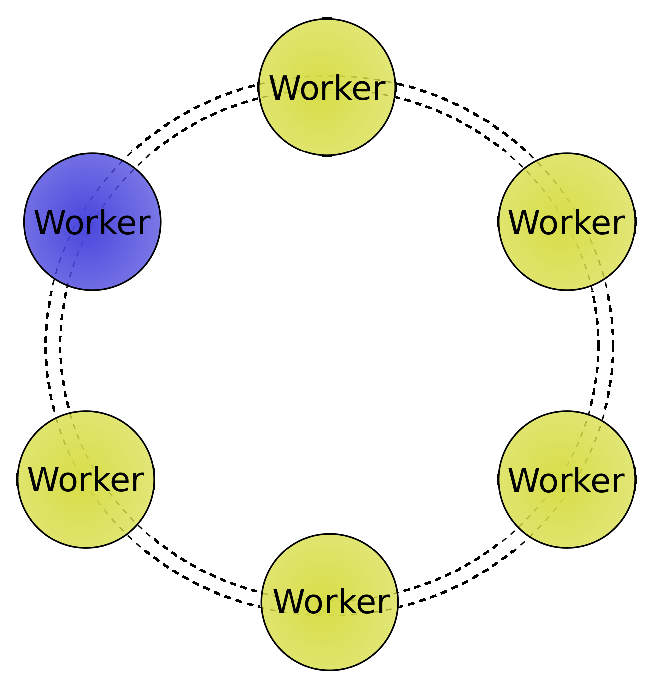
\includegraphics[scale=0.5]{pictures/All_Worker_Collective.eps}
%        }
%        \hspace{1cm}
%        \subfigure[The 0 node is assigned as the master node and handles from this on the management of the work distribution.]{%
%            \label{fig:shortColumnInCircuit}
%            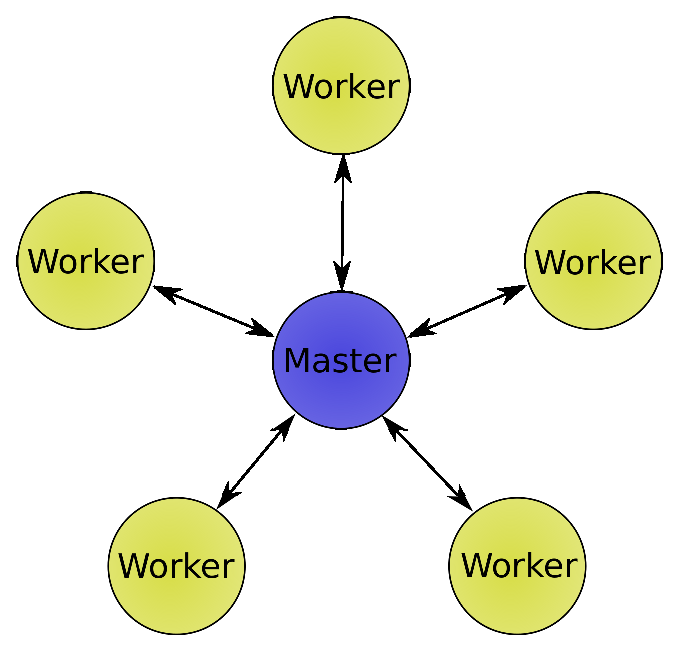
\includegraphics[scale=0.5]{pictures/MasterWorker.eps}
%       }
%    	   \end{center}
%    	\caption{%
%        The figure illustrates the work distribution and communication between the nodes.
%     }%
%   \label{fig:atlas}
%   \end{figure}

\paragraph{Load balancing}
\label{par:loadbalancing}
An efficient parallel implementation depends on a good load balancing.
The work load should be distributed equally on all ranks.
Therefore, an estimation of the work load per iteration is necessary.
But it depends mainly on the number of neurons per voxel and the distribution properties of projection densities.
Also inter process interaction influence the run times.
Each iteration can be partitioned into five parts: acceptance rejection method (\emph{linear}), storing to disk (\emph{store}),
loading experiment data (\emph{load}), select neurons in injection (\emph{selI}), select neurons in projection (\emph{selP}).
Thus, the duration per iteration, $L$, is a sum of the partial sums:
\begin{equation} \label{eq:L}
	L \approx L_{linear}(n,m,M) + L_{store}(n,\omega) + L_{load}(\mu) + L_{selI}(n) + L_{selP}(m,\mu)
\end{equation}
$L_{load}(\mu)$, $L_{selI}(n)$ and $L_{selP}(m,\mu)$ are negligible.
$\omega$ and $\frac{\partial L_{linear}(n,m,M)}{\partial M}$  can not be estimated satisfyingly.
$\omega$ represents waiting times, which occur from independent parallel write operations.
$M$ represents the distribution of probability values.
$\mu$ represents an imbalance factor.
The distribution affects the number rejections inside the linear rejection method.
Therefore, it has a significant impact on the wall-clock time.
Thus, there is only a rough estimation of the wall-clock time per voxel iteration possible.
\begin{equation} \label{eq:Lapprox}
	L_{estimate} = L_{linear}(n,m) + L_{store}(n)
\end{equation}
Therefore, a statical and dynamical voxel distribution is implemented.
At first, a third of all voxels are distributed (using Algorithm \ref{alg:distributeWeightedVoxels}) based on the weight with an estimation
of $L$ (see equation \ref{eq:Lapprox})  per voxel.
\begin{algorithm}[ht!]
\KwData{List of all voxels with weights}
\KwResult{List of private voxels and sum of weights per rank}
\For{voxel n}{
	Find rank with smallest sum of weights \\
	Add weight to sum of weights of rank \\
	\If{Rank is me}{
		Add voxel to private voxel list
	}
}
\caption{Distribute weighted voxels to ranks}
\label{alg:distributeWeightedVoxels}
\end{algorithm}

After that the master rank distributes further voxels in sets on request from the other ranks.

\paragraph{Interpolate connection information}
\label{par:interpolation}
The constant interpolation of connection information, interpolates the used experiment per voxel in 3D space.
It is implemented with an iteratively nearest neighbour search algorithm for each not injected voxel.

The algorithm iterates over all neighbours with increasing distance.
Figure \ref{longrange} shows an illustration of the search algorithm
projected in a 2D plane.
\begin{figure}[ht!]
\centering
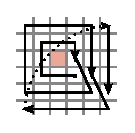
\includegraphics[scale=2.5]{pictures/longRange_Nearest_parallelAlg.eps}
\caption{Illustration of the search direction of the nearest search algorithm}
\label{longrange}
\end{figure}
The first voxel found along the search direction is declared as the nearest neighbor.
The chosen experiment from the nearest neighbour is adopted.

\subsection{Short range connections}
Algorithm (\ref{alg:BBP}) presented in the analysis section can be easily parallelized,
because each iteration is independent.
The number of generated synapses cannot be calculated beforehand.
Therefore, all synapses are stored in memory during the iterations and only written to disk 
at the end.
\begin{figure}[ht!]
\centering
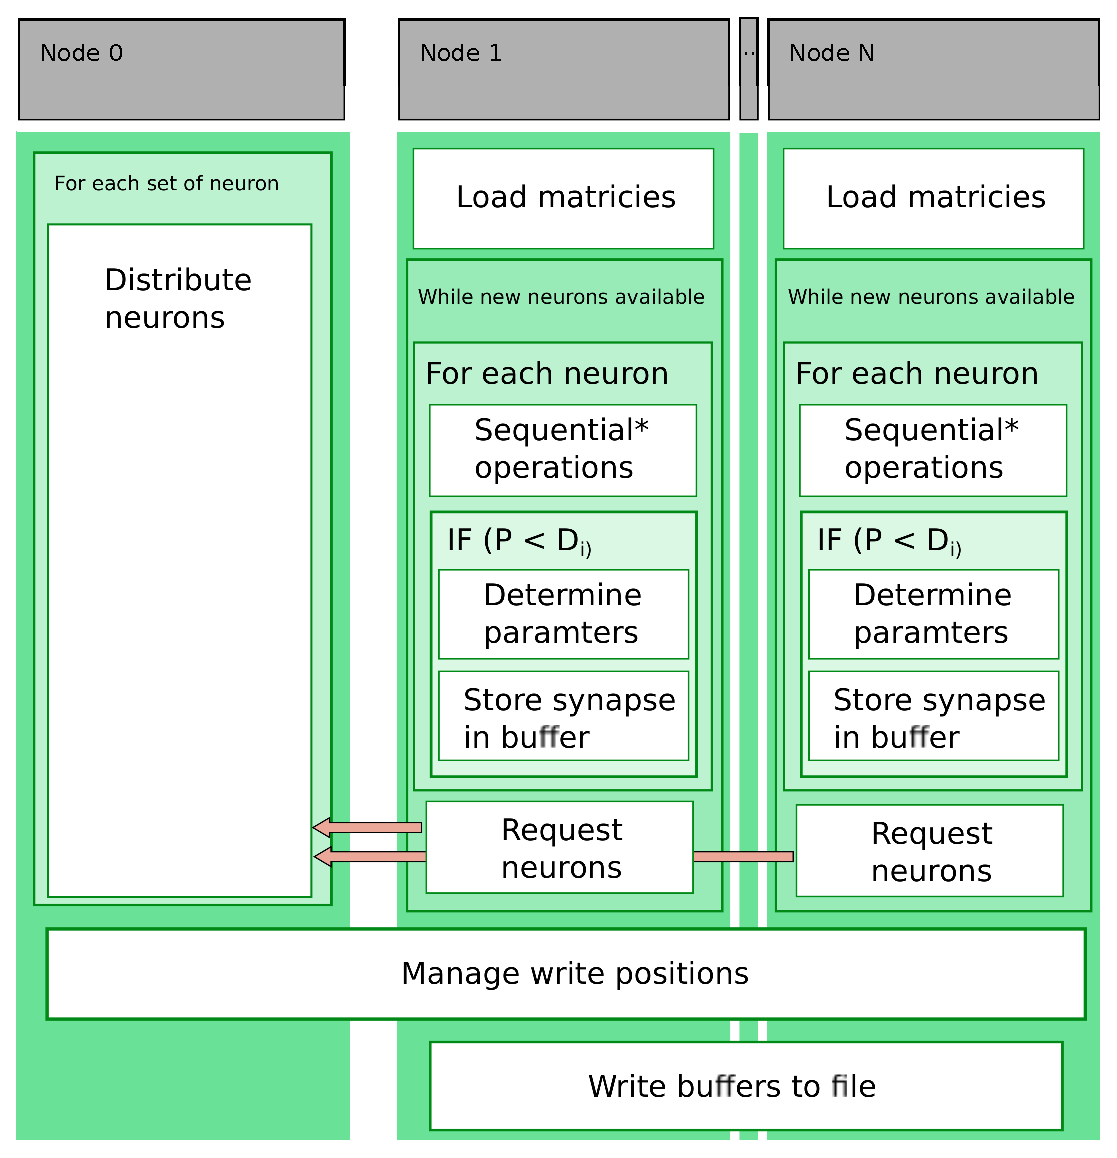
\includegraphics[scale=0.5]{pictures/shortRange_parallelAlg.eps}
\caption[Task distribution between the ranks for the short range connections generation]{Task distribution between the ranks for the short range connections generation.
It illustrates which tasks are distributed between which ranks.}
\label{fig:shortrangeparallel}
\end{figure}
The iterations from the main loop from the sequential Algorithm \ref{alg:BBP} are distributed between the ranks.
The short range algorithm (see Figure \ref{fig:shortrangeparallel}) follows the same concepts as the long range generation parallelization.
The iterations are distributed, first statically and then dynamically.
The master rank, \emph{Rank 0}, manages the dynamic distribution.
To overcome the fact that the dynamical distribution becomes a bottleneck, in the beginning a fifth of the iterations are distributed
statically between the working ranks.
The work-load per neuron is not estimated in advance.
The iterations are partitioned continuously without weights.
Each rank of the workers (all ranks except of \emph{Rank 0}) receives the neurons with the ids $x_{rank\_id-1}$
to $x_{rank\_id}$ (\emph{Rank 0} is not part of distribution. It is skipped.).
$x_i$ relates to equation \ref{eq:process2id}. It garanties a nearly equal distribution.
\begin{equation}
	x_i = round(i * \frac{N_{neurons}}{N_{ranks}-1})
	\label{eq:process2id}
\end{equation}
During runtime the master rank manages the distribution of neurons. For each neuron, 
outgoing synapses have to be created. In the first step, the workers load all needed matrices from the file system (\emph{Load matricies}).
Then, each rank requests a set of neurons from the master rank (\emph{Request neurons}). Over this set, it iterates and creates resulting
synapses. The loop from the sequential algorithm can be used (\emph{For each neuron}).
In each loop, the synapses are written to buffer (\emph{Store synapses in buffer}).
The buffer is based on its own implemented queue class. It nests standard vectors.
It contains one vector of fixed size vectors, which contain the synapse objects.
The buffer size is adapted to 
the memory available on the used IBM Blue Gene /Q systems.
At the end, the sub vectors are accessible and are written as chunks to file.
When all neurons synapses are generated, all ranks, including the master rank, calculate the writing position
in the HDF5 datasets where each rank has to write its data to (\emph{Manage write positions}). After that all workers write their synapse vectors to
disk (\emph{Write buffers to file}).


%\begin{figure}[ht!]
%   	\begin{center}
%        \subfigure[Master-worker strategy to get good balance properties]{%
%            \label{fig:shortColumn}
%            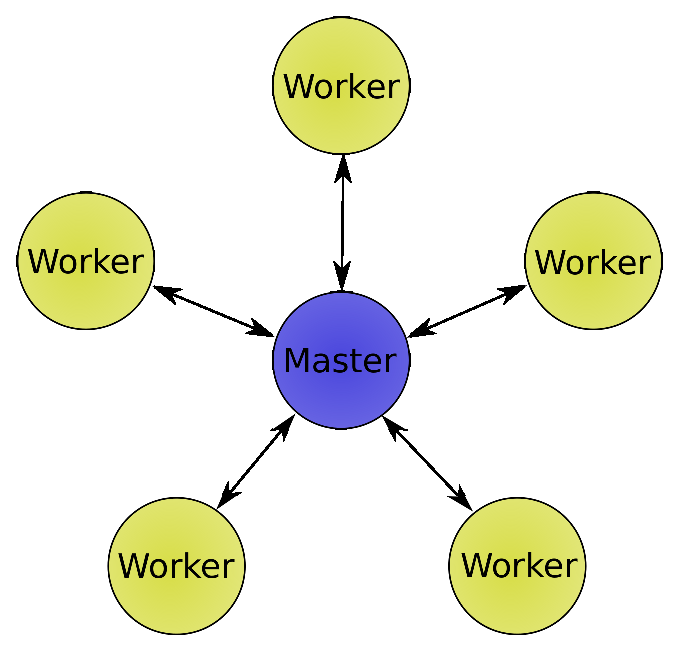
\includegraphics[scale=0.5]{pictures/MasterWorker.eps}
%        }
%        \hspace{1cm}
%        \subfigure[Collective write operation to maximize used bandwidth]{%
%            \label{fig:shortColumnInCircuit}
%            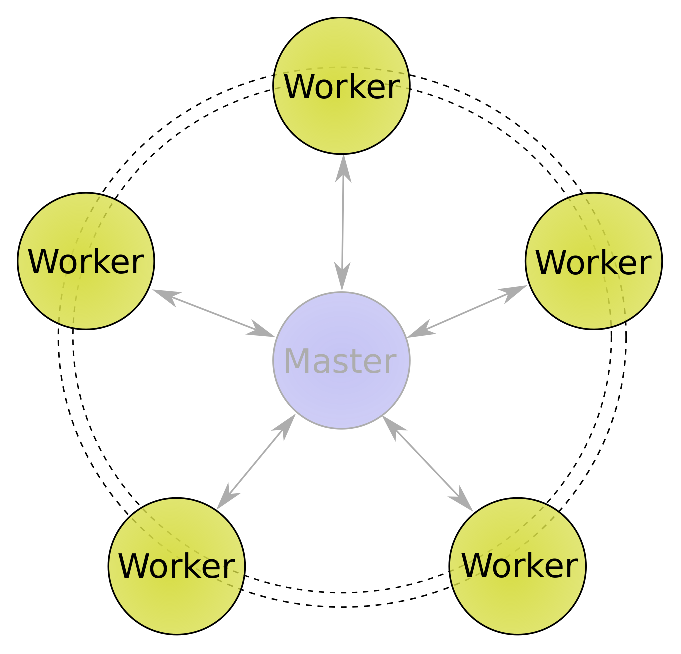
\includegraphics[scale=0.5]{pictures/Worker_Collective.eps}
%       }
%    	   \end{center}
%    	\caption{%
%        The figure illustrates the work distribution and communication between the nodes.
%     }%
%   \label{fig:atlas}
%   \end{figure}


\section{Circuit validation}
In the context of this thesis, the circuit is validated in terms of the geometrically correct placement of
the synapses. Further, the stochastic properties of the synapse files are validated.
The position of the pre-synaptic and post-synaptic neurons can be visualized and  compared to a 
reference system. For the long and the short range connectivity, the geometrical shape is known.
The long range connectivity should connect neurons from the injected regions to neurons
in the projected region for each experiment. Therefore, a circuit for a single experiment is 
generated, the pre-synaptic and post-synaptic neurons are visualized in a 3D coordinate system and the injection
and projection is used as the reference system. If pre-synaptic neurons are inside the injection space and all
post-synaptic neurons are in the projection space, the implementation is correct.

To perform the validation the renderer voxalize (see Appendix \ref{sec:voxelize}) is used.
It reduces the post-synaptic neuron cloud to densities of neurons per voxel ($N_{x,y,z}$).
The voxels can be directly compared to the projection densities ($P_{x,y,z}$) from an experiment.
\begin{equation}
	P_{x,y,z} \propto N_{x,y,z}
\end{equation}
The relation between the densities should be proportional.

For the short range connectivity, all post-synaptic neurons connected via synapses to the same pre-synaptic neuron should
lay inside a cylinder in layer 1 to 6. Visualising the post-synaptic neuron placement on top of the contour of layer 1 to
6 allows to review if the shape matches with a cylinder.
Stochastic properties were analysed with external scripts, which are not part of this thesis.

The visualization tool Paraview (see Appendix \ref{sec:paraview}) allows a visual comparison of the density values $P_{x,y,z}$ and $N_{x,y,z}$.
An example is shown in Figure \ref{fig:paraviewex}.
 \begin{figure}[ht!]
\centering
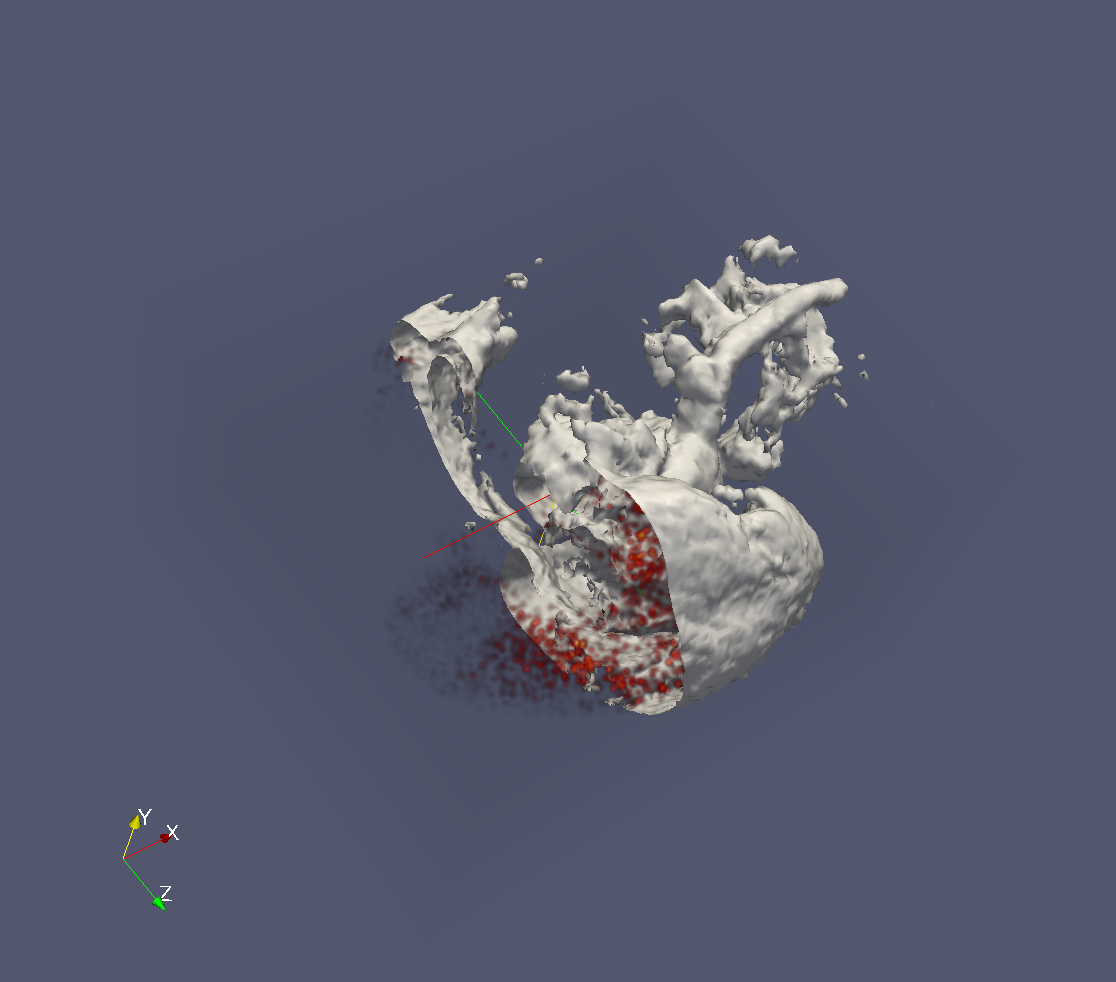
\includegraphics[width=0.4\textwidth]{pictures/paraview_ex.png}
\caption[Screenshot of Paraview]{Screenshot of a visualization with Paraview. It shows in grey the contour around the projection of an experiment.
The long range connections algorithm generated synapses only for the given experiment. 
The generated post-synaptic neurons are shown in red.}
\label{fig:paraviewex}
\end{figure}

For a visual validation, the Blue Brain Project visualization team offered a rendering pipeline to visualize the placement of post-synaptic neurons for each synapse file. Therefore, the neuron and synapse files can be imported into 
voxelize. Voxelize creates a voxelized dataset out of the post-synaptic neuron positions, which can be exported into
a MetaImage (see Appendix \ref{sec:MetaImage}) file or directly viewed with Livre (see Appendix \ref{sec:livre}).
The MetaImage files can be viewed with Paraview (see Appendix \ref{sec:paraview}).
Injection and projection images are also given in the MetaImage format.
A direct comparison inside of Paraview is possible by
loading the projection inside of Paraview and applying the contour filter on it with a threshold of $0.01$ (threshold is also applied to the same data in the long range connectivity generation). This allows to visualize the valid boundaries for all post-synaptic neurons for this particular experiment.
 
\begin{figure}[ht!]
   	\begin{center}
        \subfigure[Densities in 3D space of the projection]{%
            \label{fig:allInjections}
            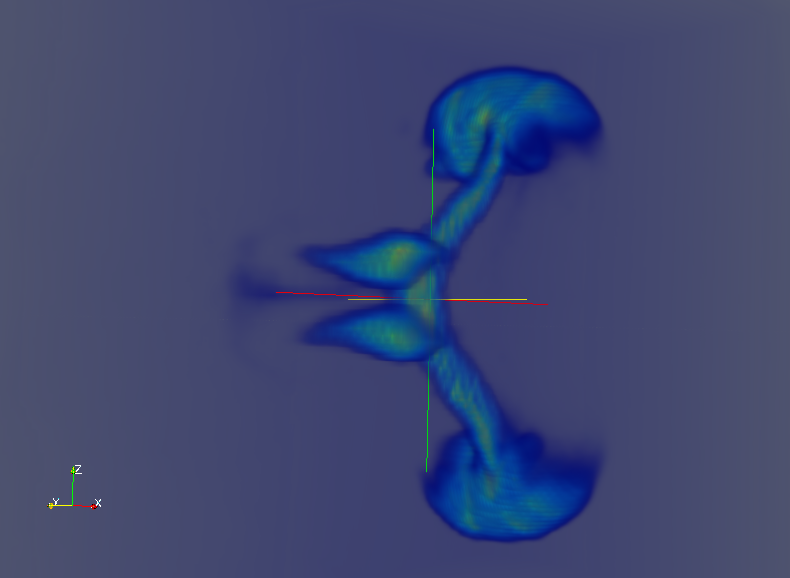
\includegraphics[scale=0.15]{pictures/exp1_energy.png}
        }
        \hspace{0.2cm}
        \subfigure[Post-synaptic neuron placement in 3D space]{%
            \label{fig:oneProjection}
            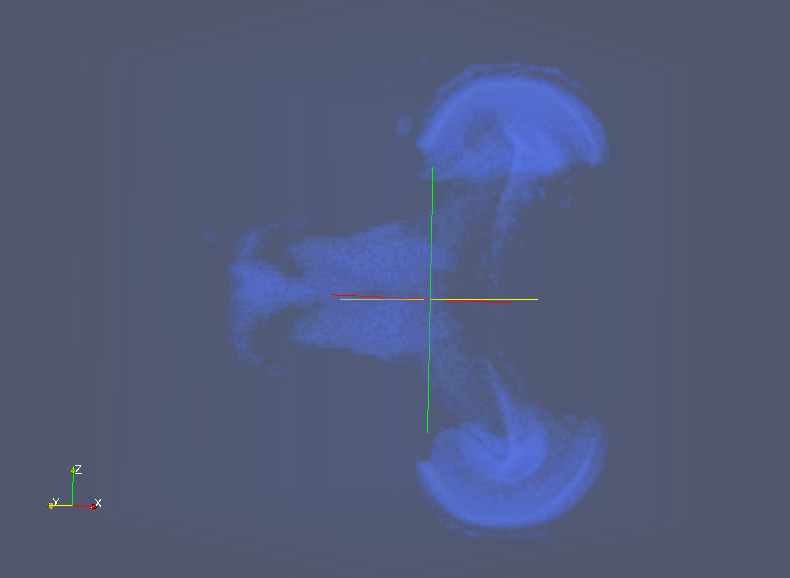
\includegraphics[scale=0.15]{pictures/exp1_post.png}
       }
       \hspace{0.2cm}
        \subfigure[Post-synaptic neuron placement inside of half cutted contour of the projection densities]{%
            \label{fig:oneProjection}
            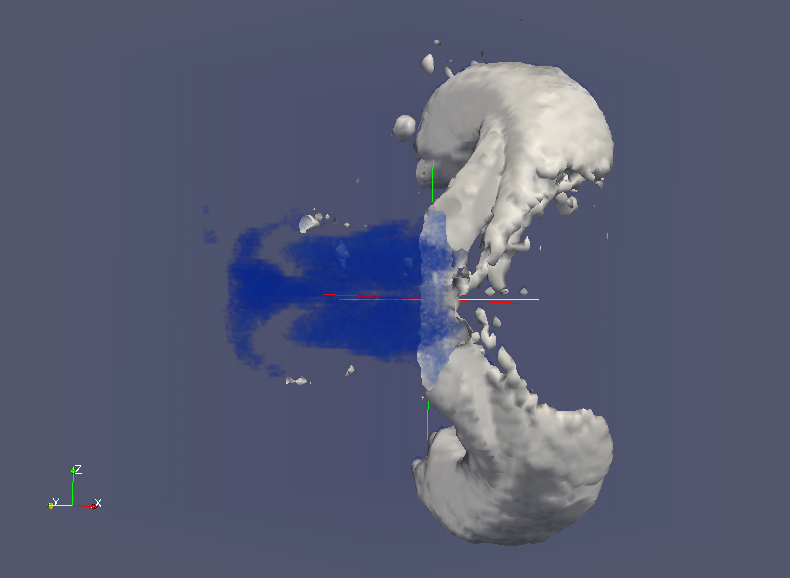
\includegraphics[scale=0.15]{pictures/exp1_post_contour.png}
       }
    \end{center}
    	\caption[Example of visual long range connections validation of a single experiment]{%
        Example of visual long range connections validation of a single experiment (id: 113935285).
        The used connections are part of the full circuit.
     }%
   \label{fig:longrangevalidation}
   \end{figure}
   
The example (see Figure \ref{fig:longrangevalidation}) illustrates the use of the visual validation of long range connections.
It shows that for the specific experiment the post-synaptic neurons are placed inside the correct regions.

Stochastic properties of the synapses parameters are validated, as well.
An analysis program iterates over all synapses in a synapse file.
The program determines min, max and mean values of all parameters.
Additionally it looks for invalid entries. An invalid entry is defined as
zero entries for all parameters. Further, he program calculates the number of in-coming
and out-coming synapses per neuron. These values are evaluated for valid boundaries.
For the long range connection generation, the out-coming synapses per neuron has to be
$0$ or $10,000$. For the short range connection generation the out-coming synapses per neuron
has to be between $0$ and $10,000$. The analysis program displays the parameter’s properties
and the number of zero entries on screen. The number of in-coming and out-coming 
synapses per neuron are written to files.
The values in the files are evaluated for valid boundaries with a Python script.



\section{NEST import modules}
The Neural Simulation Tool NEST \cite{gewaltig2007nest} is a C++ application for simulating large heterogeneous networks of point neurons. It enables the simulation of large-scale neuronal networks on super computers.
Therefore, NEST distributes the network over the available computers (see chapter \ref{sec:NEST:Datastructure}).
Each computer creates its own part of the network and only stores the synapses to its own neurons.
It uses both the Message Passing Interface (MPI) and OpenMP/Pthreads.
A large scale data-driven simulation must be integrated into the standard
workflow of NEST.
The model contains 16 TB of circuit data.
The import module for NEST should enable an efficient loading of the whole circuit.
Due to differences in the NEST internal data structure and the data delivered by the
circuit generation a transformation of the circuit data is necessary.
Synapse information contains pre-synaptic and post-synaptic
neuron ids in addition to its model parameters.
Because of the in vitro injection
methods, the synapse information maps the synapse from the pre-synaptic to the
post-synaptic neurons. For multi process simulations, NEST distributes all neurons
based on a modulo function.
Because of memory optimizations
the synapses are only stored on the post-synaptic node. This means that the
synapse information is stored on the node where the post-synaptic neuron
is located and hence it is necessary to reorder the data.
Preprocessing of the
input data should be avoided in order to maintain its original format for future changes in the circuit generation.

The internal \emph{C++} API of NEST allows the creation and manipulation of the circuit.
The API is mainly developed to work as an interface between the internal structure
and the \emph{SLI} interface. But the implementation accesses the \emph{C++} functions directly
to avoid the \emph{SLI} layer. To access the API, the internal NEST classes
have to be analysed. Because we are facing the execution on large scale machines,
we focus on thread-safty and locality of internal circuit build-up functions.
Which means, we focus on how NEST internally distributes the data, on which processes, and which
function has to be used to create a circuit inside the NEST internal data structure.


\lstdefinestyle{cppcode} {language=C++,
                basicstyle=\small\ttfamily,
                keywordstyle=\color{blue}\ttfamily,
                stringstyle=\color{red}\ttfamily,
                commentstyle=\color{green}\ttfamily,
                morecomment=[l][\color{magenta}]{\#}
                numbers=left,
  				stepnumber=5,    
  				firstnumber=1,
 				numberfirstline=true
}


%customc
\lstdefinestyle{cppcode}{
  belowcaptionskip=1\baselineskip,
  breaklines=true,
  frame=L,
  xleftmargin=\parindent,
  language=C,
  showstringspaces=false,
  basicstyle=\footnotesize\ttfamily,
  keywordstyle=\bfseries\color{green!40!black},
  commentstyle=\itshape\color{purple!40!black},
  identifierstyle=\color{blue},
  stringstyle=\color{orange},
}

\lstdefinestyle{customasm}{
  belowcaptionskip=1\baselineskip,
  frame=L,
  xleftmargin=\parindent,
  language=[x86masm]Assembler,
  basicstyle=\footnotesize\ttfamily,
  commentstyle=\itshape\color{purple!40!black},
}
\lstset{escapechar=@,style=cppcode}
%\lstset{escapechar=@,style=customc}

\subsection{Import neurons}
NEST does not support inter-process information exchange during the internal circuit building. 
To create neurons inside the circuit the identical function call has to be
performed on all ranks. NEST itself sorts out the information needed for each rank.
But by analysing NEST code, one sees that not all function calls are necessary on all ranks.
In detail, the creation (see Figure \ref{code:addnode}) of nodes (e.g neurons, subnets) has to be performed on all ranks.
\begin{figure}[ht!]
\begin{lstlisting}[style=cppcode]
/*** Add a number of nodes to the network.
   * This function creates n Node objects of Model m and adds them
   * to the Network at the current position.
   * @param m valid Model ID.
   * @param n Number of Nodes to be created. Defaults to 1 if not
   * specified.*/
  index add_node( index m, long_t n = 1 );
\end{lstlisting}
\caption{NEST internal add\_{}node function to create neurons and subnets.}
\label{code:addnode}
\end{figure}
Thus, the number of subnets and neurons have to be known on all ranks.
Calling \emph{add\_node} creates a set of nodes inside of the current subnet.
By default this is the root node of NEST.
The current subnet can be changed by calling the function \emph{go\_to} (see Figure \ref{code:goto}) beforehand.
\begin{figure}[ht!]
\begin{lstlisting}[style=cppcode]
/** Change current working node. The specified node must
   * exist and be a subnet. */
  void go_to( index );
\end{lstlisting}
\caption{NEST internal go\_{}to function to change the subnet.}
\label{code:goto}
\end{figure}
But the assignment (see Figure \ref{code:setstatus}) of model parameters can only be performed on the ranks,
where the neurons are stored.
\begin{figure}[ht!]
\begin{lstlisting}[style=cppcode]
/*** Set properties of a Node. The specified node must exist. */
  void set_status( index, const DictionaryDatum& );
\end{lstlisting}
\caption{NEST internal set\_{}status function to set model parameters of neurons.}
\label{code:setstatus}
\end{figure}
This allows to load and assign the parameters only on the corresponding ranks.
Therefore, knowing the distribution of neurons on the ranks is essential.
It can be calculated with equation \ref{eq:processfromid}.

To group neurons together with subnets, neurons can be created inside of virtual subnets.
This subnets have to be created beforehand.
Therefore, Algorithm \ref{alg:import:neurons} sorts out the needed subnets in its first step.
\begin{algorithm}[ht!]
 \KwData{HDF5 neuron dataset}
 \KwResult{Created neurons inside NEST data structure}
 Find unique values in subnet dataset; \\
 Create subnet for each unique entry; \\
 Create neurons based on length of HDF5 datasets with given neuron type inside specified subnets; \\
 Read parameter datasets collectively; \\
 Assign parameters to neurons;\\
 \hspace{0.1cm}
\caption{Import neurons from HDF5 file (see Figure \ref{fig:file:neuron}) into NEST data structure.}
\label{alg:import:neurons}
\end{algorithm}

Unique values are extracted from the subnet dataset.
After that, a subnet is created for each unique value. 
In the next step, the neurons are iteratively created inside the specified subnet.
Then needed parameter values are loaded from the HDF5 datasets and assigned to the neurons.
Derived from the distribution function (see equation \ref{eq:processfromid}), each rank has to load each $N_{ranks}$
entry starting from its rank id (the existence of subnets and in advance created nodes offset the mapping).

\subsection{Import synapses}
The synapse import module is based on the same concept as the import neuron module.
The synapse creation functionality of NEST is analysed.
Needed functions are reviewed for thread-safeness and locality.
The generated synapse files of the full mouse brain model, which have to be loaded, have a size in total of around $~16$ TB.
The total size to store the synapses in memory is of the same order as on disk (see chapter \ref{sec:NEST:Datastructure}).

To reduce the required memory size the, import synapse module should use as least amount of memory possible.
To accomplish it, the import module cannot load all synapses at once.
Thus, it has to load the synapses in parts.

The following algorithm loads the given data block-wise from disk and rearranges it into
the NEST data structure in memory.

To store a given synapse into the NEST data structure,
the NEST API function \emph{connect} has to be called.  
Different implementations are available. They vary in their argument lists.
For the given use-case we want to pass all synaptic model parameters at once and
avoid internal checks, because the implementation should cover necessary error handling by 
itself. Thus, double-checks should be avoided.
The \emph{connect} function (see Figure \ref{code:connect}) offers both functions.
It supports passing of synapse parameters and it has the least checks implemented.
Further, it accesses only objects which are owned by the executing thread. 
Therefore, it is thread-safe and can be called simultaneously from different threads.
\begin{figure}[ht!]
\begin{lstlisting}[style=cppcode]
/*** Connect two nodes. The source node is defined by its global ID.
   * The target node is defined by the node. The connection is
   * established on the thread/process that owns the target node.
   *
   * \param s GID of the sending Node.
   * \param target Pointer to target Node.
   * \param target_thread Thread that hosts the target node.
   * \param syn The synapse model to use.
   * \param params parameter dict to configure the synapse
   * \param d Delay of the connection (in ms).
   * \param w Weight of the connection. */
  void connect( index s,
    Node* target,
    thread target_thread,
    index syn,
    DictionaryDatum& params,
    double_t d = NAN,
    double_t w = NAN );
\end{lstlisting}
\caption[NEST internal \emph{connect} function to create a synapse]{NEST internal \emph{connect} function to create a synapse. The parameter list contains:
\emph{s} and \emph{target} specifies the pre-synaptic and post-synaptic neuron, respectively;
\emph{syn} is the name of the synapse model (Tsodyks model \ref{sec:dataformats});
\emph{params} contains the synapse model parameters;
\emph{d} and \emph{w} specify the synapse model delay and weight, respectively.}
\label{code:connect}
\end{figure}

It has to be called on the rank, where the post-synaptic neuron is located.
But in the file, the synapse information is grouped by pre-synaptic neurons (see chapter \ref{sec:dataformats}).
Therefore, the dataset of synapses has to be reordered before the synapses can be stored in NEST data structure.
\begin{algorithm}[ht!]
	\KwData{List of HDF5 files for each rank, block size}
	\KwResult{Connected NEST network}
	\While{Block to read in HDF5 dataset}{
		Read block and store in memory \\
 Determine target rank for each synapse \\
 Sort synapses by target ranks \\
 MPI\_Alltoallv using sorted list \\
 Connect all synapses using NEST function \\
	}
	\caption{Import synapses from HDF5 file into NEST data structure}
\label{alg:import:synapses}
\end{algorithm}

Algorithm \ref{alg:import:synapses} reads the synapses block-wise from file, rearranges (see Figure \ref{fig:importsynvis}) the order
among ranks and calls the connect function for each synapse on the corresponding rank (see chapter \ref{sec:NEST:Datastructure}).
For reference, \emph{Read block and store in memory} is called \emph{Read}, \emph{Determine target rank for each synapse} is called
\emph{Det. Node}, \emph{Sort synapses by target ranks} is called \emph{Sort}, \emph{MPI\_Alltoallv using sorted list} is called \emph{Alltoall}
and \emph{Connect all synapses using NEST function} is called \emph{Connect} from Algorithm \ref{alg:import:synapses}.
Needed initializations are grouped to \emph{Initialising}.

\paragraph{Initialising}
At first each node loads all pre-synaptic neuron references from the \emph{neuron} dataset to memory.
But each node does not need all of them. 
The neuron reference includes neuron ids (\emph{id}), number of entries  (\emph{syn\_n}) and pointers to entries (\emph{syn\_ptr}).
All entries inside the \emph{syn} dataset from  entry \emph{syn\_ptr} for \emph{syn\_n} entries have the pre-synaptic neuron specified by its \emph{id}.
\begin{figure}[ht!]
\centering
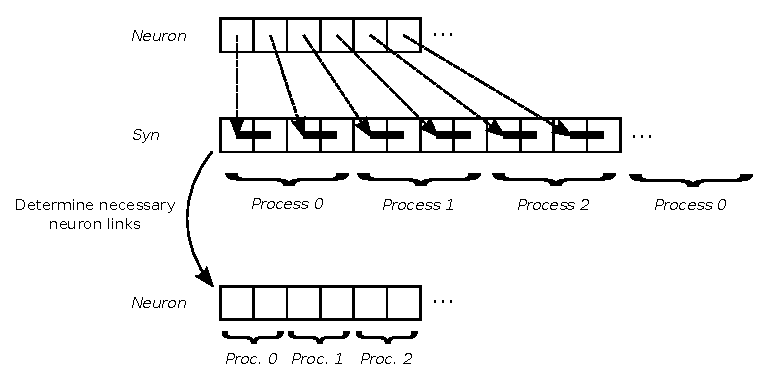
\includegraphics[scale=1.0]{pictures/NeuronLinksRemoving.eps}
\caption[Illustration of the relation of pre-synaptic neuron information to ranks]{Illustration of the relation of pre-synaptic neuron information to ranks.
By reversing the pointer specified in the \emph{neuron} dataset
each entry can be assigned to a rank.
Each rank can use it to remove unnecessary entries from memory.
}
\label{fig:neuonlinksremoving}
\end{figure}

The distribution of the \emph{syn} dataset is defined.
Each rank removes all pre-synaptic neuron references, which do not belong to
neurons inside its chunk by reversing the references (see Figure \ref{fig:neuonlinksremoving}).

\paragraph{Read step}
A block is read from the \emph{syn} dataset.
Each rank reads the entries with an offset of $N_{block} * r_{me}$ and
for each iteration it adds a stride of $N_{ranks} * N_{block}$  to the offset (e.g see first line in Figure \ref{fig:importsynvis} and \ref{fig:importsynvis2nd}).
From each entry of the block a synapse object is created
(contains pre-synaptic neuron id, post-synaptic neuron id, target neuron rank, synapse model parameters)
inside a synapse vector. Then, the pre-synaptic neuron ids are integrated into the synapse objects.

Now, each rank contains its own vector of synapses.
But most of synapses have to be stored on different ranks.
Therefore, the rank (target rank), where the post-synaptic neuron is located, is determined (using equation \ref{eq:processfromid})
and integrated.
To send it to the target rank, all synapse vectors are sorted by the target neuron rank ids.
%After that \emph{MPI\_Alltoallv} is used to send the synapses from all to all processes.
After that \emph{MPI\_Alltoallv} is used to reorder the synapses between the ranks.

Each rank receives a vector of synapses and can use the \emph{NEST} connect function to copy it to its internal data structure.
\begin{figure}[ht!]
\centering
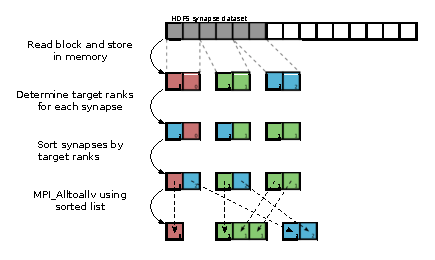
\includegraphics[scale=2.0]{pictures/import_syn_vis.eps}
\caption[Illustration of the first four steps of Algorithm \ref{alg:import:synapses} in the first iteration]{Illustration of the first four steps of Algorithm \ref{alg:import:synapses} in the first iteration.
The first row represents the \emph{syn} dataset on disk.
The following rows represent vectors of synapses per rank (represented by the column).
The color of the boxes illustrate the current association.
In the second row the association relates to the position in the \emph{syn} dataset.
Afterwards it relates to the \emph{target rank}.
}
\label{fig:importsynvis}
\end{figure}

\begin{figure}[ht!]
\centering
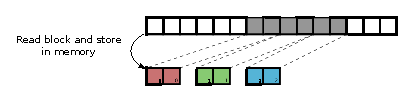
\includegraphics[scale=2.0]{pictures/import_syn_vis_second_it.eps}
\caption[Illustration of the \emph{Read} in the second iteration]{Illustration of the \emph{Read} in the second iteration.
In the second iteration each rank reads the second block of \emph{syn} dataset entries.
A block is specified as the set of read entries per iteration.}
\label{fig:importsynvis2nd}
\end{figure}
\newpage
In the last step of the algorithm, the \emph{connect} function is called iteratively for each synapse.
It is executed multi-threaded.

\paragraph{Connect step}
Each thread calls \emph{connect} for its own synapses iteratively (see Figure \ref{fig:iterateConnect}).
Synapse parameters are passed to \emph{connect} function call via a \emph{DictionaryDatum} object.
\emph{DictionaryDatum} is a SLI object for storing a map.
It uses a \emph{Token} mechanism for accessing elements.
To access entries \emph{Token} objects have to be created and deleted,
which is not thread-safe. It can produce a data race in a static memory pool object of NEST.
Therefore, the creation and deletion of the needed \emph{Token} objects are serialized with mutexes.
Besides the creation of a \emph{DictionaryDatum} object, \emph{createDictionaryDatum} creates needed \emph{Token} objects.

In between, each thread iterates over all synapses in parallel.
But each thread skips synapses where the post-synaptic neuron is not thread-local.
Thread-locality is given if $t_i$ (see equation \ref{eq:threadfromid}) is equal to the local thread id.
$i$ relates to the target neuron id.
\begin{figure}[ht!]
\begin{lstlisting}[style=cppcode]
#pragma omp parallel default(shared)
{ 
 omp_set_lock(&tokenLock);
 DictionaryDatum* d = createDictionaryDatum();  
 omp_unset_lock(&tokenLock);

 const thread tid = nest::NestModule::get_network().get_thread_id();
      
 for (int i=0;i<synapses_.size();i++) {
  try {
   const thread target_thread = getTargetThread(synapses_[i])
   if (target_thread == tid)
    singleConnect(synapses_[i], .., target_node, target_thread, ..);
   }
   catch (..) {
    ..
   }
 }
  
 omp_set_lock(&tokenLock);
 delete d;  
 omp_unset_lock(&tokenLock);
}
\end{lstlisting}
\caption[Pseudo code of thread parallel connect function calls]{Pseudo code of thread parallel connect function calls.
Parallel region executes code on all available threads.
\emph{singleConnect} function is shown in Figure \ref{fig:singleConnect}.
}
\label{fig:iterateConnect}
\end{figure}

\emph{singleConnect} assigns the parameters to the \emph{DictionaryDatum} object.
To avoid recreation of \emph{Token} objects a vector of  \emph{Token} pointers is
passed. Applying \emph{set\_{}status} on the passed \emph{Token} objects, allow to
insert the current parameters inside the \emph{DictionaryDatum} object without data races.
A loop iterates over the parameters and copies the values inside the \emph{DictionaryDatum} object.
After that the NEST \emph{connect} function is called with the pre-synaptic and post-synaptic
neuron information and the \emph{DictionaryDatum} object, weight and delay.
\begin{figure}[ht!]
\begin{lstlisting}[style=cppcode]
void singleConnect(..)
{
  index source = synapse.source_neuron;
  if (NestModule::get_network().is_local_node(target_node)) { 
    for (int i=0; i<param_names.size(); i++) {
      double value = syn.params[i] * facts[i] + offsets[i];
      setValue<double_t>( *v_ptr[i], value );
    }
    NestModule::get_network().connect(.., syn);
  }
  else {
    throw nest::IllegalConnection(..);
  }
}
\end{lstlisting}
\caption{Pseudo code of parameter assignment and NEST internal \emph{connect} function call for a single thread.}
\label{fig:singleConnect}
\end{figure}

The implementation make use of available ranks and by NEST used cores in the most compute intensive parts.
Figure \ref{fig:ConnectInsideIteration} illustrates the flow of the synapse information between ranks. 
All ranks access a single dataset to load a set. Afterwards the synapse information is processed by different steps.
In \emph{Alltoall} the synapse information are reordered between ranks.
Therefore, the synapses can be stored in the NEST data structure on the correct rank,
independently of the order in the HDF5 file.
\begin{figure}[ht!]
\centering
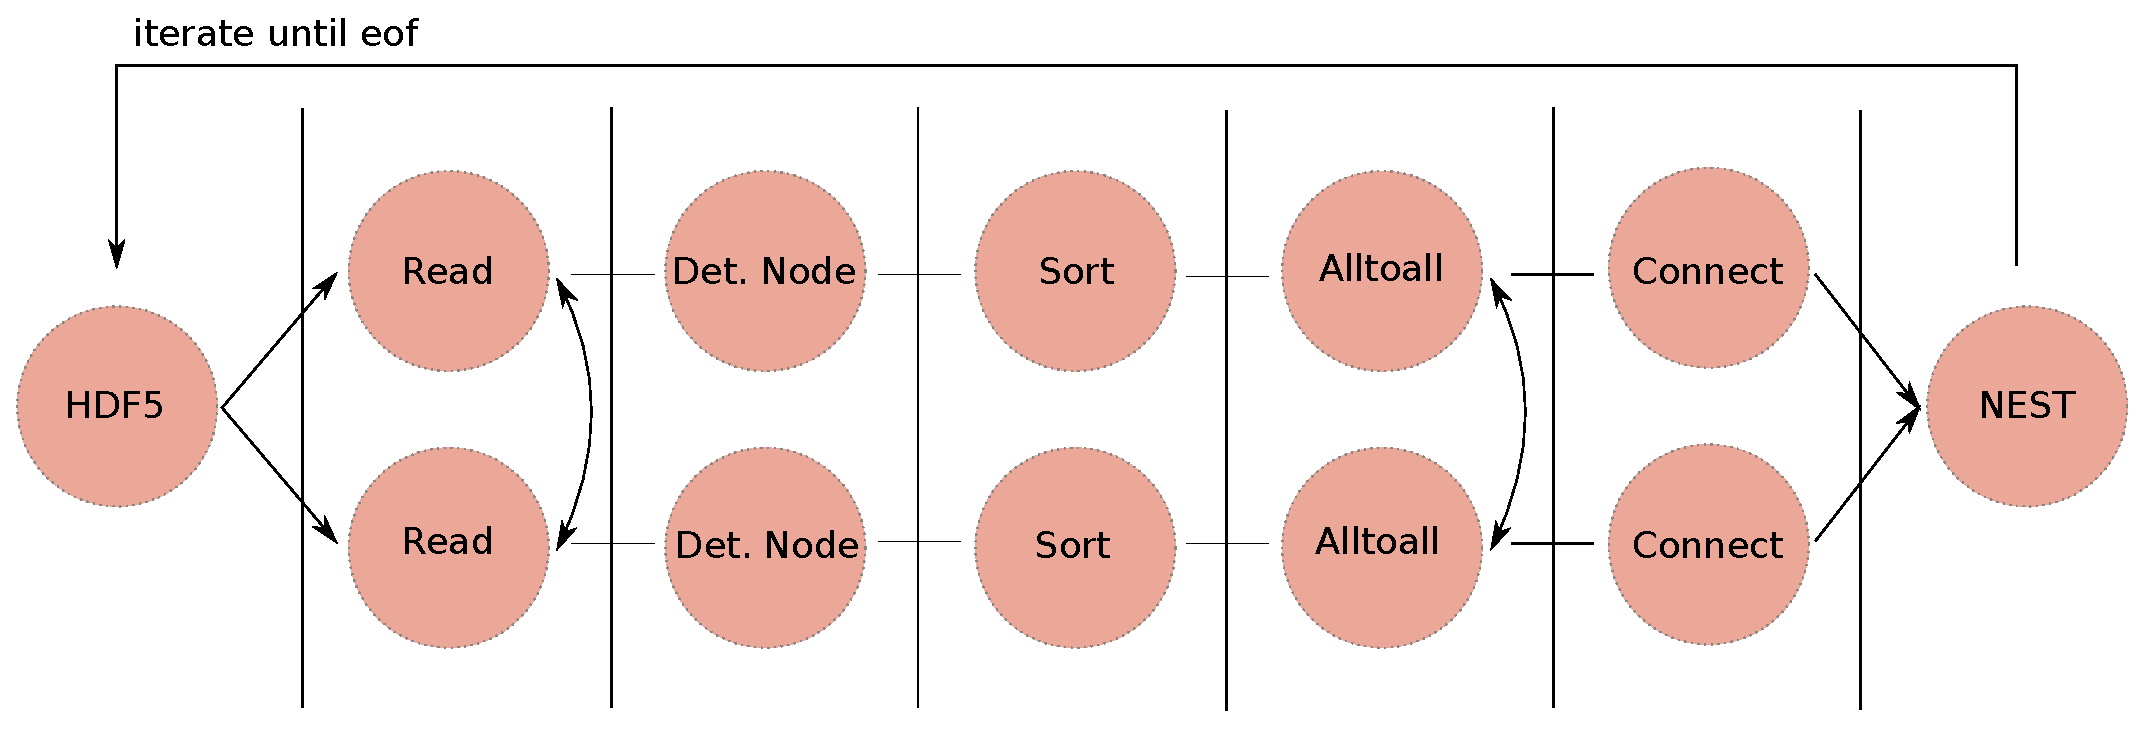
\includegraphics[scale=0.4]{pictures/Connect_inside_iteration.eps}
\caption[Illustration of synapse pipeline for two ranks]{Illustration of synapse pipeline for two ranks. It shows how the synapse information is processed by each tasks and when collective operations are performed.
The two rows represent two parallel processes.}
\label{fig:ConnectInsideIteration}
\end{figure}
\newpage
\subsection{Memory consumption}
NEST stores the whole mouse brain model in memory.
The data-driven simulation is limited by its memory consumption.
The neurons import module does not need to be memory efficient.
It is executed before all synapses are stored in memory.
During execution most of the given memory is free, which is more than needed.
The import synapse module shares the memory with the synapses inside the NEST data structure.
The theoretical memory consumption is analysed:
\begin{table}[ht!]
\centering
\begin{tabular}{| l | l | l | l |}
    \hline
    step & memory consumption \\ \hline \hline
    Init & $\nu * N_{neurons} * sizeof(neuron)$ \\ \hline
    Read & $\nu * N_{neurons} * sizeof(neuron) + N_{block} * sizeof(synapse)$ \\ \hline
    Det. Node & $\nu * N_{neurons} * sizeof(neuron) + N_{block} * sizeof(synapse)$ \\ \hline
    Sort & $\nu * N_{neurons} * sizeof(neuron) + N_{block} * sizeof(synapse)$ \\ \hline
    Alltoall & $\nu * N_{neurons} * sizeof(neuron) + 2 * N_{block} * sizeof(synapse)$ \\
    &$ + \sim N_{block} * sizeof(synapse)$ \\ \hline
    Connect & $\nu * N_{neurons} * sizeof(neuron) +  ~N_{block} * sizeof(synapse) $ \\ \hline 
    \end{tabular}
\caption[Theoretical memory usage of each step of the load synapse module]{The table lists the theoretical memory usage of each step of the load synapse module.
$\nu$ corresponds to the distribution of pre-synapic neurons between the ranks.
$N_{neurons}$ relates to the number of pre-synaptic neurons available in the dataset.
$N_{block}$ relates to the size of the loaded block.}
\label{tab:stepmemory}
\end{table}
The maximal memory consumption can be taken from Table \ref{tab:stepmemory}.
The approximated maximal memory consumption is given by:
\begin{equation}
 M_{max} \approx \nu * N_{neurons} * sizeof(neuron) + 3 * sizeof(synapse)
\end{equation}
$N_{block}$ is adaptable.
An appropriate buffer size for the import synapse module can be calculated.
The buffer size is equivalent to the block size.
The import synapse module should use less than $5\%$ of the total available memory per rank.
The implemented buffer is a standard vector of \emph{Synapse} objects.
The \emph{Synapse} objects are defined as in Figure \ref{fig:synapsebuffer} shown.
\begin{figure}[ht!]
\begin{lstlisting}[style=cppcode]
struct Synapse
{
  unsigned int pre_neuron;
  unsigned int post_neuron;
  unsigned int rank_id;
  double prop_values[5];
}
\end{lstlisting}
\caption[Pseudo code of \emph{Synapse} struct]{Pseudo code of \emph{Synapse} struct.
\emph{pre\_neuron} contains the pre-synaptic neuron id.
\emph{post\_neuron} contains the post-synaptic neuron id;
\emph{rank\_id} contains the target rank id;
\emph{prop\_values} contain the synapse parameters;
}
\label{fig:synapsebuffer}
\end{figure}

An optimal buffer size is determined via test runs.
The theoretical optimal value is equal to the block size of the file size.
For the JUQUEEN system the file system block size is $4$ MB.
Several runs using different buffer sizes around $4$ MB are performed.
\begin{figure}[h!]
\begin{center}
 \includegraphics[width=0.7\textwidth]{pgfplots/findBuffer.pdf}
\end{center}
\caption[Bandwidth comparison of the import module using different buffer sizes]{Bandwidth comparison of the import module using different buffer sizes.
Multiple runs are preformed with 8 (blue dots) and 16 (red squares) on JUQUEEN.}
\label{schumann:fig:findBuffer}
\end{figure}
The achieved bandwidth (see Figure \ref{schumann:fig:findBuffer}) is relatively constant for block sizes between $4$ and $30$ MB on $8$ and $16$ racks.
We implement a standard block size of $12$ MB.
